\documentclass[11pt,a4paper,twoside]{report}

%%%% Packages
\usepackage{a4wide}
\usepackage{graphicx}
\usepackage{lmodern}
\usepackage{fancyhdr}
\usepackage{titlesec}

\usepackage{times} % assumes new font selection scheme installed
%\usepackage{amsmath} % assumes amsmath package installed
%\usepackage{amssymb}  % assumes amsmath package installed
%\usepackage{color}  % assumes amsmath package installed
%\usepackage[pdftex]{hyperref}
%
\usepackage{url}
%\usepackage{ulem}

\usepackage{enumitem}
\usepackage{pdfpages}

\graphicspath{{../../../pictures/logos/}{.}}



% % % % % % % % % % % % % % % % % % % % % % % % % % % % % % % % % % % % % % % % 
% % % % % % % % % % % % % % % % % % % % % % % % % % % % % % % % % % % % % % % % 
% Definitions -- TO BE UPDATED FOR EACH DELIVERABLE
%
\newcommand{\wpnumber}{WP 7}

\newcommand{\delnumber}{D7.3}
\newcommand{\deltitle}{Guidelines for software development}
\newcommand{\delversion}{0.1}

\newcommand{\deldate}{January 31st, 2013}
\newcommand{\delnature}{Report}
\newcommand{\delpublic}{Public}

\newcommand{\delauthors}{Author 1 (Institution) \newline
                         Author 2 (Institution)}


% % % % % % % % % % % % % % % % % % % % % % % % % % % % % % % % % % % % % % % %
% Project-wide definitions
%
\newcommand{\grantnumber}{288533}
\newcommand{\projectacronym}{ROBOHOW.COG}
\newcommand{\projecttitle}{Web-enabled and Experience-based Cognitive Robots
                           that Learn Complex Everyday Manipulation Tasks}


% % % % % % % % % % % % % % % % % % % % % % % % % % % % % % % % % % % % % % % % 
% % % % % % % % % % % % % % % % % % % % % % % % % % % % % % % % % % % % % % % % 
% Page headers and title page (do not edit!)

% \titleformat*{\chapter}{\Large\sffamily}
\titleformat{\chapter}[display]{\bfseries\Huge}{\Huge Chapter \thechapter}{1ex}{}
\titleformat*{\section}{\Large\sffamily}

% page headers
\pagestyle{fancy}
\setlength{\headheight}{14pt}
\lhead{\sffamily\delnumber}
\chead{\sffamily FP7-ICT-\grantnumber \ \projectacronym}
\rhead{\sffamily\today}


\begin{document}
\sffamily

% title page
\begin{titlepage}

  \begin{center}
  %  \includegraphics[width=8cm]{logo-robohow.pdf}
  %  \\[3cm]
    \textbf{
    \textsf{\huge  ICT Call 7}\\[0.5cm]
    \textsf{\huge \projectacronym}\\[0.5cm]
    \textsf{\huge FP7-ICT-\grantnumber}\\[2cm]
    \textsf{\Large Deliverable \delnumber :}\\[0.5cm]
    \textsf{\Large \deltitle}}\\[3cm]
  \begin{figure}[h!]
  \centering
  %\includegraphics[width=5cm]{logo-FP7.pdf}
  \end{figure}
  \vfill
  \textbf{\textsf{\large \today}}
  \end{center}
\end{titlepage}

% page 2
\begin{center}
\begin{tabular}{ p{0.3\textwidth} p{0.6\textwidth} }
  Project acronym:      & \projectacronym\\
  Project full title:   & \projecttitle\\
  \\
  Work Package:         & \wpnumber  \\
  Document number:      & \delnumber \\
  Document title:       & \deltitle  \\
  Version:              & \delversion\\
  \\
  Delivery date:        & \deldate\\
  Nature:               & \delnature\\
  Dissemination level:  & \delpublic \\
  \\
  Authors: & \delauthors\\

\end{tabular}
\end{center}

\flushleft
The research leading to these results has received funding from the European 
Union Seventh Framework Programme FP7/2007-2013 under grant agreement
n$^\textrm{o}$\grantnumber \ \projectacronym.

\tableofcontents
% % % % % % % % % % % % % % % % % % % % % % % % % % % % % % % % % % % % % % % %
% % % % % % % % % % % % % % % % % % % % % % % % % % % % % % % % % % % % % % % %
% % % % % % % % % % % % % % % % % % % % % % % % % % % % % % % % % % % % % % % %





% % % % % % % % % % % % % % % % % % % % % % % % % % % % % % % % % % % % % % % % 
% START EDITING HERE

%\chapter*{Summary}
%Summary....
%
%
%\chapter{Chapter-Title}
%
%\section{Section 1.1}
%
%\section{Section 1.2}

%\title{}
%\maketitle
%\tableofcontents
%
\pagebreak

This document will detail some rules for future developed code.
Keep in mind that the code will be read by humans and will be eventually modified by them (you may not be the last person to use it). 
It must be readable, understandable and reusable.\\

The most important rule about coding is the \textbf{consistency}.
Hence, ifa project already has its own format, do not impose yours, and try to adapt yourself.
There are several reasons for that:
\begin{itemize}
\item Correcting everything will take you a long time that you may not have
\item If you are a visitor/occasional developer of a package, you may signal to the main developers that some rules have been broken. But don't do it by yourself, temporarily mixing two coding styles is not a good thing to do.
\end{itemize}
Prefer asserting the consistency inside one package rather than the consistency inside the whole project.
However, if you are creating a new package, please follow those coding guidelines.

\chapter{General guidelines}
\label{section:general-guidelines}
\begin{itemize}
\item Ensure the consistency of each project (this is \textit{that} important).
\item Maintain the documentation up-to-date (use doxygen, sphinx...), and make your code understandable.
\item Make the validation of the code easier by adding unit-tests.
\item Use versioning tools (git or svn, depending on the type of data), tag versions that work and release often.
\item Keep the code clean. Remove useless and dead code (especially if it is versioned).
\item Do not neglect debugging tools (e.g. make the debug easier by using assertion (C++)).
\end{itemize}

\section{General shape of package}
A package should at least contain the following elements:
%The general shape of a package is as follow:
%General shape of packages (like, a Readme, folder structure - include - src ...)
\paragraph{Readme.md}
The readme.md file is the first file a newcomer will consult. 
It should define all the informations relative to the project:
\begin{itemize}[noitemsep,topsep=0pt,parsep=0pt,partopsep=0pt]
\item The purpose of the package.
\item The use/compilation informations: on which OS does it work? What are the dependencies of the project (with the version if it matters).
\item The related papers.
\item The origin of the sources, and the project management web application (github, redmine \ldots) 
\end{itemize}

\paragraph{Authors}
The list of contributing authors can be added at the top of each files.
The order to keep is the alphabetical order of last name, then first name.

Since this can be a daunting task, an alternative is to define an AUTHOR file in the root directory of your package, in which you can indicate the corresponding(s) author(s) and list all the contributors and a summed up detail of their contribution.\\

\paragraph{Copyright}
The full text statements of all licenses used in the project should be placed in the LICENSES directory at the top of the repository.
If you add a package under a license that is not included in LICENSES, add the license statement.

The code developed in the frame of the robohow project should be open source.
The licenses used in this purpose are the following ones (from the more restrictive to the least one).
\begin{itemize}
\item GPL\footnote{\url{http://www.gnu.org/licenses/gpl.html}}, permits the use of the library only for free programs.
\item LGPL\footnote{\url{http://www.gnu.org/copyleft/lesser.html}} permits the use of the library in proprietary programs.
\item BSD \footnote{\url{http://opensource.org/licenses/BSD-3-Clause}}
\end{itemize}

% According to ROS guidelines\url{http://www.ros.org/wiki/DevelopersGuide}

\section{Clarify and document your code}
Keep in mind that your code will be read, reused and (eventually) improved by humans.
You want them to use your code wisely, and you don't have the time to help each of them personally.

Write the documentation and the code at the same time. 
Detail the how of your code, but don't forget the why. 
Knowing the goal of your code will help one to detect/correct wrong behavior.

Do not hesitate to detail any specific or unusual implementation
(e.g. the use of the specific structure of a sparse matrix to gain computation time).
Similarly, document your variables: units, specific bounds, legal values and give them \textit{explicit} names (avoid \begin{tt}tmp\end{tt} or random sequence of letters).	

Please refer to the articles corresponding to the code, \textit{especially} if the notations come from it.

Yet, do not overload your code by documenting the obvious. This can be avoided:\\
\begin{tt} i+=1 //increase the index value of 1\end{tt}

\section{Test a lot}
Testing is the easiest way to check the behavior and good health of your code through its evolution.
It allows to find what (and who) is responsible for a wrong behavior.
Also, it can also be of help to understand the code.

The sooner the tests are added to the project, the easier it is to debug it.
Similarly, the more automatized it is, the better.
\begin{itemize}[noitemsep,topsep=0pt,parsep=0pt,partopsep=0pt]
\item Do unit tests (verifies the behavior of the code)
\item Do regression tests (verifies that the behavior of the code do not change with the evolution of the code)
\item Do computation time tests to find bottleneck in your code (e.g. use callgrind in C++ )
\item Do memory handling tests (valgrind).
\end{itemize}

Automatize your tests using cTest or gtest\footnote{\url{http://www.ros.org/wiki/gtest}}.

\section{Bug tracking - bug report}
Eventually, you'll encounter some issues using code developed by someone else.\\
Do not hesitate to report an issue, and to signal the issue in the code with a TODO.\\
Please be explicit when you report an issue, and define the following informations:
your goal (maybe there is another/safer way to do what you're trying to do), 
your OS (32 bits/64 bits), your version of ROS, the version of the packages you are using...\\

Prefer opening a ticket on the project management web application associated to the package, than contacting directly the person in charge of the code. 
You might not be the only one to encounter the problem and the resulting discussion might help someone else.\\

Help the developers to reproduce the bug, e.g. by creating a branch corresponding to your problem.

%\note{voir la liste des choses à ne pas faire pour plus de détails}


\section{Feature request}
Similarly to the bug report, prefer opening tickets on the corresponding website.
You can help someone by doing this, especially when there are reasons not to implement the proposed feature.

\section{Deprecation}
As soon as there are users of your code, you have a responsibility not to pull the rug out from under them with sudden breaking changes. 
Instead, use a process of deprecation, which means marking a feature or component as being no longer supported, with a schedule for its removal. Give users time to adapt, which is usually one release cycle, then do the removal.

%Deprecation can happen at multiple levels, including:
%
%\begin{verbatim}
%
%API features : Say you want to remove a method call from a library. First mark it as deprecated in the API documentation; with DOxgyen, use @deprecated. If the language supports it, also mark the code as being deprecated; in C/C++, use __attribute__ ((deprecated)). In the next release, note the deprecation in the ChangeList, with the future release at which you expect to remove it; if it's a widely used feature, make the deprecation notice prominent, and explain the reasoning behind it. In that future release, remove it.
%Packages : Say you want to remove a package. Mark it as deprecated in the Wiki documentation (e.g., put DEPRECATED at the top), with a note as to when you expect to remove it. Include notice of the deprecation in the ChangeList with the next (stack) release. If it's a widely used package, you should also send mail to your users giving them as much advance warning as possible.
%\end{verbatim}

\chapter{Versioning general settings}
% Whether it is for a private project or a shared project, it is mandatory that ones uses a versioning tool.


\section{SVN or Git?}
Use Git for text files, e.g. sources code (C, python, matlab, java...) or latex (.tex, .bib).\\
You may use SVN for huge binary-like files (.doc files, videos, pdf...). 
Indeed, using git to version huge files will drastically increase the size of the local git repository on the user's side. With svn, you can do only partial checkout, which can be practical.\\

Define the files to be ignored by using .gitignore or svn:ignore. 
Typically, \textbf{never version restricted access file} or automatically generated files (e.g. by a compiler).
If you add by mistake such files, contact your administrator so that he can correct this quickly before anyone pulls it.
% \url{http://svnbook.red-bean.com/en/1.1/ch07s02.html#svn-ch-7-sect-2.3.3}

%\section{Naming convention}
%
%The naming convention is the one proposed by git :
%\begin{verbatim}
%name = FirstName LastName
%\end{verbatim}

\section{Commit message}

It is important to keep the commits as small and simple as possible.
Typically, create one commit per topic (bug fix, feature addition,  documentation update...).
Do NOT mix up bug fixing and feature addition, this will make the commit impossible to understand.
This will increase the readability and make the cherry-picking and the debugging (e.g. with \begin{tt}git bisect\end{tt}) easier.
Hence, do not use \begin{tt}git commit -a\end{tt}, prefer adding the files one by one or only chosen parts of files in your commit (using \begin{tt}git add -p\end{tt}).

\paragraph{Reverting commits}

Sometimes, a wrong commit can be pushed, by mistake or inattention.
Before reverting a wrong commit, please contact its author so as to know if it is possible for him to correct his mistake or if he can revert himself.
If the author cannot be reached and the revert is necessary and urgent (e.g. the main branch does not compile any more and external users need it), please indicate the reason of the revert. 
It can help the author of the commit to understand this decision, and avoid reverts of revert.

\paragraph{Convention}
Commit messages should be written in English in the present tense 
(so as to match up with commit messages generated by commands like \begin{tt}git merge\end{tt} and \begin{tt}git revert\end{tt}.)
They should have the following shape:
\begin{verbatim}
Brief description of the commit (< 60 characters)

Thorough description of the commit.
- item 1
- item 2
\end{verbatim}

When correcting a bug, define the bug tracker reference (if any) and/or the bug origin or a small description of it.
Please avoid putting simply "Remove bug".\\

When committing code on behalf of others use the \begin{tt}{--author}\end{tt} option, e.g. \begin{tt}git commit --author "Emmett Brown $<$\url{emmett.brown@bttf.org}$>$"\end{tt},
or thank the person in the message "Thanks to Emmett Brown for notifying."

\section{Tag}
Tagging is a really handy way to ensure the coherence of a set of packages, e.g. by using pkg-config.
The release tags have the shape vX[.Y[.Z[-descr]]] (eg. 1.0, 0.2.3-beta)

\begin{itemize}[noitemsep,topsep=0pt,parsep=0pt,partopsep=0pt]
\item X is the major version number. Change of major version number indicates that the code may not be backward compatible.
\item Y is the minor version number. It indicates an improvement that should be backward compatible.
\item Z is the patch version (bug fix or security fix) 
\item desc corresponds to the beginning of the git commit id.
\end{itemize}

It is also possible to define tags for specific purpose (experiments, paper...).
In this case, they can have a different shape (eg: iros2012-FirstAuthorName).\\


Prefer tagging with a message, in order to get the correct tag with \begin{tt}git describe\end{tt}.\\
Also, you can use the -s option to create a GPG-signed tag and certifies that \textit{you} are the one that created the tag.

\begin{tt}
\$ git tag -s v1.2.3 -m"Small description"\\
\$ git describe\\
> v1.5.1-2-g59d2 \# where 59d2 is the commit number.\\
\$ git tag -v v1.2.3\\
object f148df68ed4f5c1fb7d35aae68342f6bb0ab7356\\
type commit\\
tag v1.2.3\\
tagger Emmett Brown <emmett.brown@bttf.org> 1357239557 +0100\\
~\\
Small Test\\
gpg: Signature made Wed 21 Oct 2015 07:59:17 PM CET using RSA key ID 8D7EAAA1\\
gpg: Good signature from "Emmett Brown <emmett.brown@bttf.org>"\\
\end{tt}
~\\
For SVN, the tag command is:\\ 
\begin{tt}svn cp --parents <repo>/trunk <repo>/tags/v0.0.1\end{tt}\\

%	\note{When creating the tag for a demo, make sure that all the required files can be found.}
~\\
ROS has a specific stack version policy \footnote{\url{http://www.ros.org/wiki/StackVersionPolicy}}:
\begin{itemize}[noitemsep,topsep=0pt,parsep=0pt,partopsep=0pt]
\item 0.1: completely experimental, unreviewed
\item 0.2: some review has occurred, and we are migrating this stack to more stable APIs
\item 0.3: ready to start including with distributions, though definitely not stable
\item 0.4-0.8: on stable development cycle towards 1.0 release (aka tick-tock)
\item 0.9: 1.0 release candidate
\end{itemize}


\section{Branch}
The main branch, \textbf{master}, should \textbf{always} be usable (compilable and executable with unit tests successful).
Another branch, \textbf{stable}, contains all the stable versions of the code.

Except from small modifications, all developments should be first realized in a separated branch (that may be published or remain local), tested, then merged with the master branch.\\


\paragraph{Convention}
The name of the branch should describe the purpose of the branch.
Sorting the branches by sub-folders (i.e. using '/') increases the readability for a high number of branches.

Branches in the root folder (such as "master", "stable", "iros02"...) should be usable whereas 
work in progress should be in a sub-folder (e.g. topic/debug-dynamic, \textit{developer-name}/dev for a personal branch).

\paragraph{Branch or tag?}

Use a tag if you are sure that the corresponding commit is usable and stable.
Otherwise, use a branch, so as to allow adding patches afterwards, and make the update of local repository easier.




\subsubsection{Merging branches: git rebase and git merge}

Consider the project with two branches \textit{initial} and \textit{feature} on your local machine.
Two commands, \begin{tt}git rebase\end{tt} and \begin{tt}git merge\end{tt}, can be used to gather the modifications realized in the two branches.
They differ in the way the blending is realized, as depicted in Fig.~\ref{fig:merge-rebase}:
\begin{itemize}
\item The merge process consists in keeping the history of both branches and creating an additional commit entitled "Merge branch ..." that gathers the modifications of both branches.
\item The rebase process consists in reapplying all the commits of the current branch after the last commit of the target branch. 
 For example:\\
\begin{tt}
emmet@pc:\textasciitilde/work (feature): git rebase initial\\
\end{tt}
will stack all the commits of the feature branch after the commits of the master initial, and will rewrite the feature branch.
% This could be compared to the application of git cherry-pick on each commit of the current branch.
\end{itemize}


\begin{figure}[htb]
\centering
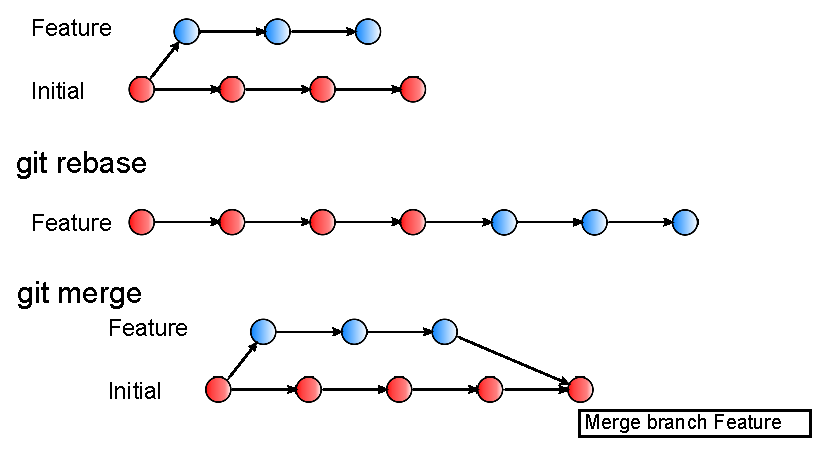
\includegraphics[scale=1]{img/merge_rebase.eps}
\caption{Difference between the commands \textit{git merge} and \textit{git rebase}.
The first graph represents the original state of the git repository.
The second one shows the result of the command \textit{git rebase initial}, realized on the branch \textit{feature}: the shape of the branch feature changes, so that every commit realized on this branch now appear to be realized after the commits realized on the init branch
The third graph shows the result of the command \textit{git merge feature}, realized on the branch \textit{initial}: an extra commit, gathering all the modifications realized on the branch feature, is added to the branch initial.}
\label{fig:merge-rebase}
\end{figure}

If you are afraid of losing the initial branch after a rebase (e.g. if one step of the rebase went wrong), do the rebase from a temporary branch\\
\begin{tt}
emmet@pc:\textasciitilde/work (feature): git checkout -b rebase-feature\\
emmet@pc:\textasciitilde/work (rebase-feature): git rebase origin initial
\end{tt}\\
You can also retrieve the initial branch using \begin{tt}git reflog\end{tt}.

The advantage of the rebase process is to keep the history readable and more linear.
As a consequence, browsing the history and debugging (using \begin{tt}git bisect\end{tt}) is simpler.
In exchange, the initial history is rewritten (order of commit modified, commits squashed...).\\

The advantage of the merge is that it keeps the original order of the commits.
The main disadvantage is that the history graph will quickly grow into a bag knot, making debugging a nightmare, especially when several users develop on the same branch.
Also, in case of conflict, the resulting commit is likely to be really obscure if some extra modifications have to be added.\\


In order to have a more linear history, it is better to use \begin{tt}git rebase\end{tt}, especially for small differences (1 to 3 commits).\\

\section{Communication with remote repository}

Working with a remote repository introduces some subtleties and some extra good practices to follow.
Since this repository is likely to be shared between several users / several places, it is 
important to ensure the good state and the coherency of the remote repository.
An error realized on this repository may be hard to correct and is likely to propagate quickly.
It is thus important to know what to do and what not to do.\\

Especially, the good use of the command \textit{git rebase} requires a little practice, 
so if you are not familiar with this command, 
please ask the maintainer of the code to realize the merge/rebase operation for you.

\subsection{Recommended practices}
\subparagraph{Forbidden practices}
Briefly, it is forbidden to modify a commit that has already been pushed. 
Such operations are likely to damage the remote repository and/or the repository of other users.
In particular, the following practices should be prohibited: 
\begin{enumerate}
\item Forcing a push. \textbf{Never} use the command \begin{tt}{git push -f}\end{tt}
\item Changing a commit after pushing it. Once pushed, it is too late to do a \begin{tt}{git commit --amend}\end{tt} (this commands allows to correct a commit by changing the commit message or the modifications included).
\item Rebasing a branch already on the remote repository, and pushing again on this branch, ie:\\
\begin{tt}
git branch feature origin/feature $\#$ create the branch feature.\\
git checkout feature		$\#$ change to the branch feature\\
git rebase master		$\#$ change the order of commits\\
git push origin feature  $\#$ Push the modifications to the remote branch (not straightforward in most cases).\\
\end{tt}
 
The rebase process should be done only at the very end of the life cycle of a branch.
Rebasing published branches can lead to duplicate commits in the shared repository. An exemple is given in section~\ref{section:rebase-warning}.
\end{enumerate}

The only exception to the rule 1 is when a file that should not been distributed has been pushed (file containing a password, sensitive informations \ldots).
In this case, you can destroy the wrong commit by using \begin{tt}push -f\end{tt} and/or contacting the main person in charge of the code to explain what happened.

\subparagraph{Good practices}
Before pushing on the remote repository, it is important to make sure that all the required files are included, and that everything works well: 
clone your repository in a local folder (e.g. /tmp/), then compile and test it.
This simple manipulation reduces small mistakes such as forgotten files.


\subsection{Merging of branches}

The life and death of a branch follows classicaly this scheme, illustrated by Fig.~\ref{fig:life-and-death}
\begin{enumerate}
\item Create the branch \textit{topic/feature} based on the branch \textit{start}\\
\begin{tt}
git pull origin start\\
git checkout -b topic/feature
\end{tt}

\item Add some commits.

\item  Occasionally, merge with the starting branch\\
\begin{tt}
git pull origin/start
\end{tt}

\item At the very end (before the merge), rebase against the starting branch \\
\begin{tt}
git rebase origin/start
\end{tt}

\item  Do not forget to test the new branch.\\

\item  Go back to the starting branch and \textbf{merge} with the branch to be deleted.\\
\begin{tt}
git checkout start\\
git merge topic/feature
\end{tt}

\item  Delete the branch\\
\begin{tt}
$\#$ delete remote branch\\
git remote prune feature\\
git push origin :refs/heads/feature\\
$\#$ delete local branch\\
git branch -D feature
\end{tt}
\end{enumerate}

\begin{figure}[htb]
\centering
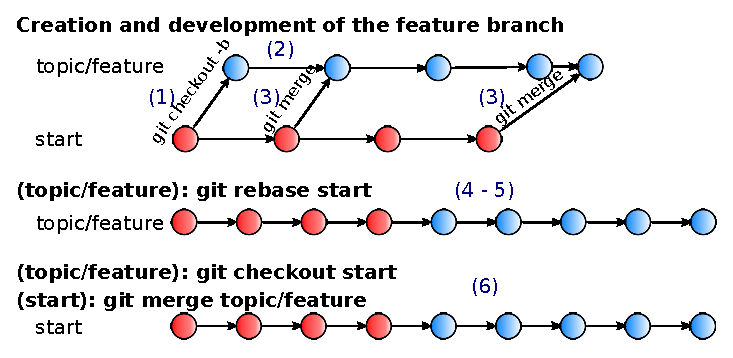
\includegraphics[scale=1]{img/life_and_death.eps}
\caption{Life and death of a feature branch.}
\label{fig:life-and-death}
\end{figure}

%If required, check with the local authority.

\subsection{Rebasing during branch update}

The rebase appends when one wants to gather two branches, but also during the update of a branch.
When both the local and the remote repositories have been modified, the user has to update his
locate repository before being authorized to push his modifications.
Using the command \begin{tt}git pull\end{tt} will implicitly realize a merge between the remote and the local branches if the pull is not feed-forward.

To avoid creating knots in the history graph, prefer using \begin{tt}git pull --rebase\end{tt} instead of \begin{tt}git pull\end{tt}. 
Note that to avoid (bad) surprises, you can do it in several steps:\\
\begin{enumerate}[noitemsep]
\item \begin{tt}git pull origin current\_branch\end{tt} ~~~
 \# do the merge: you can then check that everything went well.
\item 
\begin{tt}git rebase  origin/current\_branch\end{tt}  ~~~
 \# stack your modifications after those in the remote repository.
\end{enumerate}
 
Also, the following commands can be of use:
\begin{tt}git fetch \end{tt} checks if there are any modification of the remote repository.\\
\begin{tt}git pull -ff-only \end{tt} pulls the remote modifications only if the pull is feed-forward (else fails).\\




\subsection{Cleaning up}

Do not forget to clean the dead branches of the remote repository from time to time.
\begin{tt}
\# Delete tracking branch\\
git remote prune name\_of\_remote\_branch\\
\# Pour supprimer une branche :\\
git push origin :refs/heads/name\_of\_remote\_branch
\end{tt}

% Remote repository interaction.
% git pull, push, rebase.
% Branch and pull
% … take advantage of git stash.
% Git submodule. Git ignore ?


\subsection{Warning on git rebase}
\label{section:rebase-warning}

As explained earlier, the git rebase is a powerful tool enabling to have a clean history, which make the debugging easier. 
However, when you rebase a branch, it is likely that its shape will differ of the shape of the corresponding branch on an remote repository. 
As a consequence, it is forbidden to continue working with this remote branch, because of readability reasons.\\
%As a result, it is now forbidden to push again the branch $B\_local$ on the branch $B\_remote$:
%because of the change of history, it is now impossible to realize a push just after the rebase (the push is not straightforward). You will have to pull the remote branch, which will realize an automatic merge.
%As a result, some commits will be present twice in the history, making it unreadable.



The figure~\ref{fig:rebase-warning} illustrates the evolution of the local branch \textit{feature}, that is rebased on the branch \textit{start} and merged again with the remote branch \textit{origin/feature}.
Before the rebase operation, the remote repository and the local repository are identical.
We realize a \textit{git rebase start} on the branch feature: the commits of the branch feature are now placed after the commits of the branch \textit{start} (Figure~\ref{fig:rebase-warning}B).
The content of the commits "K" and "L" are the same\footnote{For simplification reasons, let's assume that no conflict occurred during the rebase}, but their id are now different (illustrated by the change of color).\\

Starting now, the remote branch and the local branch have a totally different structure. 
Hence, it is not possible to push the branch feature on the remote branch (the push is not straightforward).
In order to push on the remote branch, it would be necessary to update your local repository, that will create the tree illustrated in Figure~\ref{fig:rebase-warning}C. 
As a result, the repository will contain the commits "K" and "L" twice, making the history unreadable.

Since that without this discouraged merge process, it is no longer possible to communicate with the remote branch origin/feature, the best solution would now be to create a new remote branch with a different name (origin/feature2) or to merge the modification with the start branch (if it is the end of the branch cycle).


\begin{figure}[htb]
\centering
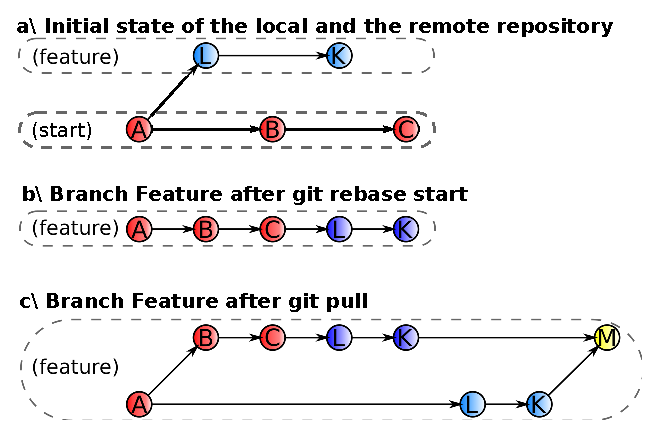
\includegraphics[scale=1]{img/rebase-warning.eps}
\caption{Wrong behavior: pulling a branch after rebasing it leads to the duplication of the history.}
\label{fig:rebase-warning}
\end{figure}








\section{Structure of a GIT repository}
The repository should follow the model proposed in \footnote{\url{http://nvie.com/posts/a-successful-git-branching-model/}}.
%\begin{figure}
%\includegraphics[width=0.95\columnwidth]{Git-branching-model.eps}
%\caption{Structure of a GIT repository}
%\end{figure}
Here is a short summary:
\paragraph{Main permanent branches}
The repository should have two permanent branches:
\begin{itemize}
\item The \textit{master} branch, that contains commits as small as possible. This branch gives the detailed history of all the modification that have been realized on the repository. 
\item The \textit{stable} branch, that contains released version only. They \textbf{must} work. The corresponding commits may be huge, since they correspond to squashes of commits that have been pushed in the develop branch.
\end{itemize}

\paragraph{Extra permanent branches}
Other permanent branches can be created, corresponding to important demonstration or papers.
Those repositories should be stored in the root of the git repository.

\paragraph{Temporary branches}
Next to those branches, other branches can be created for several reasons:
\begin{itemize}
\item Develop new features. At the end of the test process, the commits \textit{must be rebased} with the release branches. Since the rebase can be tricky, please ask the code maintainer to do it if you are not familiar with this command.
\item Develop a hotfix. Once done, that are merged with both the master and the develop branch. 
%\item Develop a release. Once done, that are merged with both the master and the develop branch. 
\end{itemize}

\paragraph{Bug fixes}
Bug fixes can be cherry­picked into the stable branch.



\begin{figure}
\includegraphics[width=0.95\columnwidth]{img/Git-branching-model.eps}
\end{figure}



%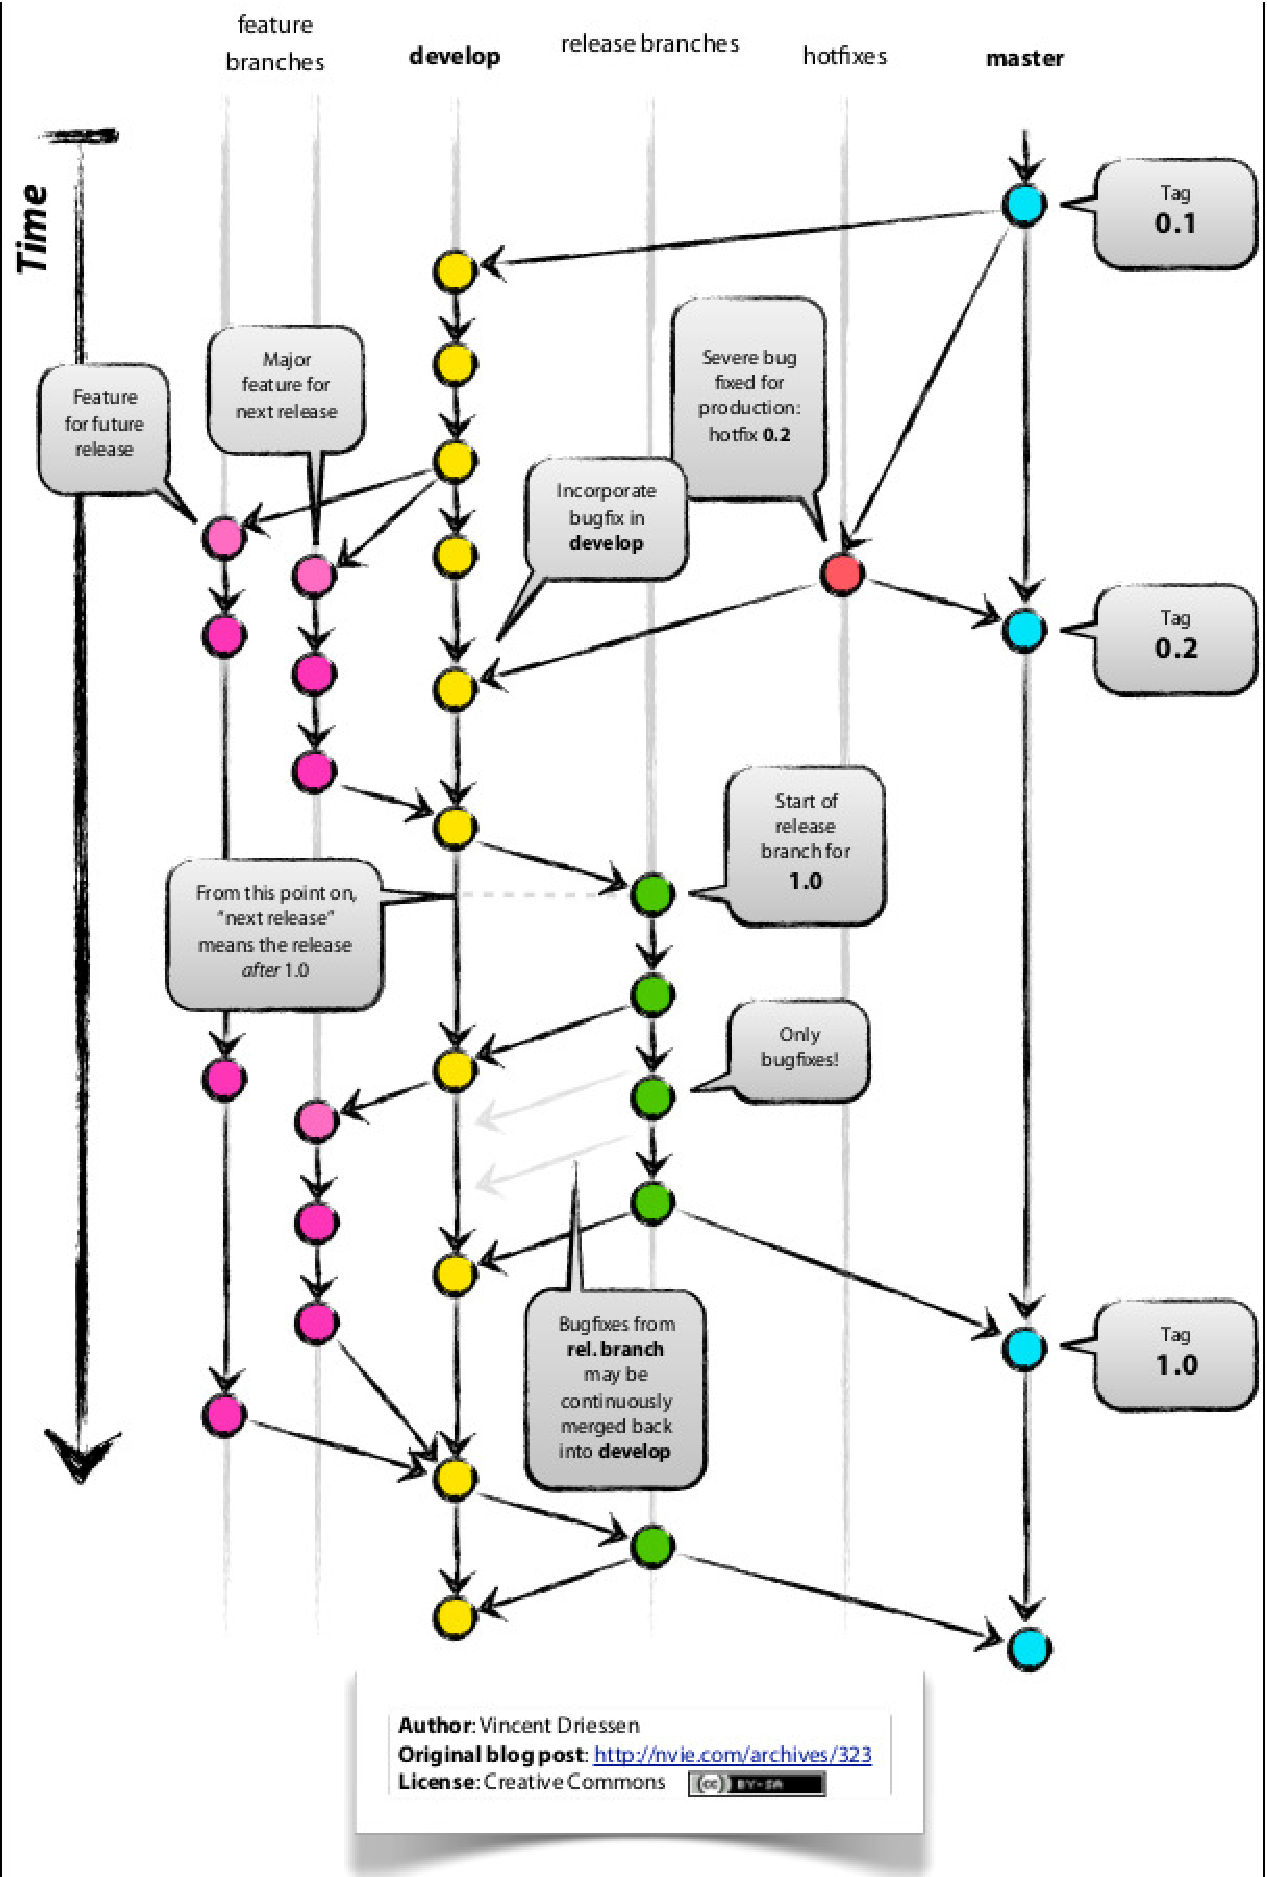
\includepdf[pages={1}]{img/Git-branching-model.pdf}

%\paragraph{Rebasing huge branches}
%\note{Robohow fellows: I'd like your opinion on the following issue:}
%The policies "every commit of the master can be computed" and "Use git --rebase" may conflict, especially 
%when the branch merged with the master branch is huge.
%Two solutions are possible:
%\begin{itemize}
%\item use the possibilities offered by git rebase to modify the commits (e.g. squash them).
%\item realize a merge with the master, so as to purposefully create a "circuit". 
%This offers the possibility to explore the commits realized in the branch (while ensuring that every commit in the master branch is functional).
%\end{itemize}


\section{Working in community}

\paragraph{Modifying an external package}
If you have write access to the remote repository, you can commit your modification, push them in a new remote branch (\begin{tt}git push origin patch/improvement\end{tt}), ask for verification from the main developers that will do/authorize the merge with the master branch. \\


If you do not have write access to the remote repository, commit the modification on your local repository and create the corresponding patches using the command 
\begin{tt}git format-patch reference\_commit -o out\_folder\end{tt}\\
e.g. 
\begin{tt}git format-patch origin/master -o patches\end{tt}

This command will convert all the commits from the reference\_commit to the last one into applicable commits,
and store them in the folder \textit{patches}

Thus, the main developers will be able to directly apply your patches using the command
\begin{tt}git apply patch\end{tt}\\

\textbf{Do NOT} do \begin{tt}git diff > patch.txt\end{tt}
This will create a file that is not directly usable, and the developers will have to recode your modifications.

\paragraph{Using others' packages}
Prefer working with stable branches or tagged versions, that are more likely to be stable, and are better reference points.



\section{Sources}

\paragraph{General guidelines}~\\
\small{\url{https://wiki.duraspace.org/display/FCREPO/Git+Guidelines+and+Best+Practices}}\\
\small{\url{http://goo.gl/H5OnA}}\\

\paragraph{Commit message shape}~\\
\small{\url{http://tbaggery.com/2008/04/19/a-note-about-git-commit-messages.html}}\\

\paragraph{About the merge and the rebase}~\\
\small{\url{http://darwinweb.net/articles/the-case-for-git-rebase}}\\
\small{\url{http://jeffkreeftmeijer.com/2010/the-magical-and-not-harmful-rebase}}\\
\small{\url{http://nvie.com/posts/a-successful-git-branching-model}}\\
%\end{document}
\pagebreak
\section{ROS guidelines}

The following rules are a copy of the slides created by Lorenz M\"osenlechner \footnote{\url{https://robohow.org/_media/meetings/first-integration-workshop/ros-best-practices.pdf}}.\\

The ROS libraries are by default installed in the /opt/ros folder. 
\textbf{Never} edit those files. Prefer using ROS overlays \footnote{\url{http://www.ros.org/wiki/fuerte/Installation/Overlays}} instead.
Use the tool support \textit{rosws} to create, modify and manage overlays.
Multiple overlays with different versions can exist in parallel, e.g.:
\begin{itemize}
\item Overlay for development.
\item Overlay for demos.
\item Overlay for experimenting with bleeding edge code of other people.
\end{itemize}

\subsection{ROS Overlays}
\paragraph{Creation}
The creation of an overlay with rosws is realized as follows:
\begin{verbatim}
sudo pip install rosinstall #Install rosws
rosws init ~/fuerte /opt/ros/fuerte # Create a new overlay
# Load the created file setup.bash in .bashrc (optional)
# echo "source ~/fuerte/setup.bash" >> ~/.bashrc 
\end{verbatim}

\paragraph{Add packages}
To add a local directory (e.g. a sandbox for experimental packages), do:
\begin{verbatim}
mkdir ~/fuerte/sandbox
rosws set ~/fuerte/sandbox
\end{verbatim}

\paragraph{Installation}
Install packages from a rosinstall file:
\begin{verbatim}
rosws merge robohow-cram.rosinstall
rosws update
\end{verbatim}
Install a (released) stack from source:
\begin{verbatim}
roslocate info turtlebot | rosws merge -
rosws update
\end{verbatim}

The rosinstall files correspond to a YAML description of repositories to install.
They are ideal for repository snap shots and collaboration, and enable to specify versions, e.g:
\begin{verbatim}
- git:
   local-name: cram_pl
   uri: http://code.in.tum.de/git/cram-pl.git
   version: 0.1.5
- svn:
   local-name: knowrob
   uri: http://code.in.tum.de/pubsvn/knowrob/tags/latest
\end{verbatim}


\subsection{Naming Conventions}
\paragraph{File names}
\begin{itemize}
\item Package names are lower case.
\item Packages and stacks must not contain dashes (“-”), only underscores (“$\_$”).
\item Messages, services and actions are named in camel case:
\begin{tt}geometry\_msgs/PoseStamped \end{tt}
\item Do not use the word “action” in an action definition (e.g.: Foo.action, not FooAction.action).
\end{itemize}

\paragraph{Topics, parameters, actions, services}
\begin{itemize}[noitemsep]
\item Nodes, topics, services, actions, parameters are all lower case with underscores as separator.
\item Never use global names, always node local topic, service, action and parameter names. 
\item Use ros::NodeHandle handle("\textasciitilde")\\
\begin{tabular}{ll}
\textbf{Bad} & \textbf{Good}\\
ros::NodeHandle nh();         & ros::NodeHandle nh("\textasciitilde");\\
nh.advertise$<$Foo$>$("foo", 10); & nh.advertise$<$Foo$>$("foo", 10);\\
Topics: $\rightarrow$ /foo &
Topics: $\rightarrow$ /node\_name/foo
\end{tabular}
\end{itemize}


\subsection{Best Practices}
\paragraph{Topics vs. Services vs. Actions\\}
\begin{itemize}
\item Use \textit{topics} for publishing continuous streams of data, e.g. sensor data, continuous detection results, . . .\\
\item Use \textit{services} only for short calculations.\\
\item Use \textit{actions} for all longer running processes, e.g. grasping, navigation, perception, . . .
\end{itemize}


\paragraph{ROS package}
\begin{itemize}
\item ROS packages are cheap, create many.
\item One package per functionality.
\item Create separate packages that contain only messages, services and
actions (separation of interface and implementation).
\begin{itemize}
\item Keep your dependencies clean:
\item only depend on what you need
\item specify all dependencies 
\item do not use implicit dependencies
\end{itemize}
\item Provide launch files.
\item Group packages in stacks.
\end{itemize}


\paragraph{Misc}
\begin{itemize}
\item Use standard data types when possible.
\item Do not define matrix data types for transforms but use geometry\_msgs/PoseStamped.
\item Do not require a specific startup order for nodes: use \begin{tt}waitForService\end{tt}, \begin{tt}waitForTransform\end{tt}, \begin{tt}waitForServer\end{tt}, . . .
\item Use ros::Time, ros::Duration and ros::Rate instead of system time.
\item Do not use command line parameters but the ROS parameter server.
\item Use rosconsole utilities for logging (ROS\_INFO, ROS\_DEBUG, \ldots).
\item Never call cmake by hand in a package!
\end{itemize}


\subsection{Third Party Libraries}
\begin{itemize}
\item If possible, try to use libraries from Debian packages.
\item Specify rosdep dependencies (tool for installing system packages).
\item If you need to compile a library from source create a ROS wrapper
package that downloads and compiles the package.
\item Don't use sudo in wrapper packages.
\item Don't require manual system wide installations.
\item Don't copy libraries into packages that need them.
\end{itemize}


\subsection{Collaboration}
% Use version control systems (e.g. git or svn)
% Create tags for stable versions that others can use.
\begin{itemize}
\item Provide a rosinstall file.
\item Create a short Wiki page for each package:
\item Document what the node does.
\item Document topics, services and actions that are required and
provided.
\item Document ROS parameters and their default values.
\item Data can be recorded and exchanged using bag files.
\end{itemize}

\subsection{ROS Bag Files}
%\note{definition of a ros bag}
Recording of a bag:
\begin{tt}rosbag record <topic> <topic> ...\end{tt}\\
Play a bag:
\begin{tt}rosbag play foo.bag\end{tt}\\
Play a bag using recorded time (important when stamped data and
TF was recorded):\\
\begin{tt}rosbag play --clock foo.bag\end{tt}




\pagebreak
\section{Code guidelines}

%For each of the following langage, I may invite the reader to follow an existing guidelines, in which case I will briefly sum the most important do and don't rules.
%Also, I propose to add some exceptions / tolerated elements.

The integration in ROS is one possible objective of the code.
As a result,  the first guidelines proposed are those of ROS.
However, please be aware that this integration is not mandatory: one can wants its code to be used outside of the ROS framework and independently from any middleware.

%However, keep in mind maintaining that the consistency of code style in each package has priority above all other consideration.
%Follow this guide whenever possible, e.g. when creating a new package, but if you are editing a package written by someone else, follow the existing stylistic conventions in that package.


Some general guidelines have already been given in the section 1.\note{ref...}.
The following rules refine them for some coding languages.
Some pointers will be given for extra reading.

% \subsection{General guidelines}
% ?

\subsection{CPP guidelines}

The cpp guidelines are those given by ROS.
Hereafter are gathered some of the most important guidelines:

\paragraph{Convention}
C++ source files have a .cpp extension, header files a .h extension.\\
The files are named in lower case, using underscores:\\
\begin{tt}
my\_package/include/my\_package/foo\_bar.h\\
my\_package/src/foo\_bar.cpp\\
\end{tt}

\begin{itemize}
\item Files defining a class have the name of the class.
\item C++ classes/types are normally named in camel case:\\
\begin{tt}
class FooBar { ... };
\end{tt}
\item Functions are in \begin{tt}camelCase\end{tt}, and their arguments are under\_scored\\
\begin{tt}
int exampleMethod(int example\_arg);
\end{tt}

\item Variables are \begin{tt}under\_scored\end{tt}.

\item Constants are all capital: \begin{tt}GRAVITY\_FORCE\end{tt}.
\end{itemize}

\paragraph{Variables}
Make your variable name explicit.
Avoid one-letter variables, except for integral iterator variables (i, j, k).
Avoid using tmp, aaaa or meaningless random sequence of letters.
An exception is tolerated if the notation come from a paper (matrix name etc). 

\paragraph{Namespace}
Use namespaces to scope your code and gather classes/methods that belong to a same package or topic.
Avoid defining global variables / functions. 
Define them in an appropriate namespace or in an anonymous namespace in the cpp file to limit their effect.

\paragraph{Headers}
The headers mus be protected by multiple inclusion by using \#ifndef guards
\begin{verbatim}
#ifndef PACKAGE_PATH_FILE_H
#define PACKAGE_PATH_FILE_H

#endif  //PACKAGE_PATH_FILE_H
\end{verbatim}

Keep the headers light: use forward declaration.\\
Never add "using namespaces" in headers

\paragraph{Class}
Attributes of class should have a final underscore to distinguish them from other variables.
%Avoid protected?
Forbid the copy of classes when necessary by making the copy constructor private or making the class inherit from : boost::noncopyable
Do not abuse of the friendship.

\paragraph{Function}
Output arguments to methods / functions (i.e., variables that the function can modify) are passed by pointer, not by reference.\\
Heavy Object should be passed by const reference, except for small data (bool, char, int, double)\\
\begin{tt}
int exampleMethod(const FooThing \& input, BarThing* output);
\end{tt}

\paragraph{Be a const addict} Add const whenever it is possible: in the parameters of a function (input/output) and for methods that must not modify the class attributes.\\
Return elements by const reference.\\
Do not return by const copy (it does not make sense).
\begin{verbatim}
const std::vector<double> & getValue() const; // Good
const std::vector<double>   getValue() ; // Bad
\end{verbatim}


\paragraph{Preprocessor macros} should be avoided. Prefer inline functions, enums, and const variables to macros.

\paragraph{Debugging and testing}
Use assertions: assert or ROS\_ASSERT (for code on ROS).\\
Use Ros messages: ROS\_FATAL, ROS\_ERROR, ROS\_WARN, ROS\_INFO, ROS\_DEBUG.\\
Use callgrind, valgrind.

\paragraph{Exceptions}

Exceptions are the preferred error-reporting mechanism, as opposed to returning integer error codes.\\
Always document what exceptions can be thrown by your package, on each function / method.\\
Don't throw exceptions from destructors.\\
Don't throw exceptions from callbacks that you don't invoke directly.\\


When your code can be interrupted by exceptions, you must ensure that resources you hold will be deallocated when stack variables go out of scope. In particular, mutexes must be released, and heap-allocated memory must be freed. Accomplish this safety by using the following mutex guards and smart pointers:

\paragraph{Forbidden practices}~\\
Do NOT ignore warnings. If some warnings are way too verbose (e.g. boost on windows), silent them one by one.



\paragraph{Sources}~\\
Ros: \url{http://www.ros.org/wiki/CppStyleGuide}\\
google: \url{google-styleguide.googlecode.com/svn/trunk/cppguide.xml}\\
Forbidden Practices: \url{http://www.strauss.za.com/sla/code_std.asp}\\




\subsection{Python}
I propose to follow the python guidelines given by ROS \url{}

\paragraph{Indentation} Use 4 spaces per indentation level.

\paragraph{Parentheses} should be use sparingly: do not use them in return statements or conditional statements unless using parentheses for implied line continuation. %(See above.) It is however fine to use parentheses around tuples. 

\paragraph{Imports} should usually be on separate lines, e.g.:
\begin{verbatim}
Yes: import os
     import sys

No:  import sys, os
\end{verbatim}

It's okay to say this though:\\
\begin{tt}
from subprocess import Popen, PIPE
\end{tt}

\paragraph{Note on compatibility}
Use the REAL types returned by the function you use.
\begin{enumerate}
\item Example 1: Python/C API\footnote{\url{http://docs.python.org/c-api/dict.html}}\\
\begin{tt}Py\_ssize\_t PyDict\_Size(PyObject *p)\end{tt}\\
If you use this function you \textbf{MUST} use a Py\_ssize\_t and not an
integer type chosen by you.
Failing to do so will create conversion errors on different platforms.

\item Example 2: Matrix Libraries and STL containers
\footnote{\url{http://www.cplusplus.com/reference/stl/vector/}}

A vector size method has the following API:
\begin{tt}size\_type size() const;\end{tt}

Which means that the size *MUST* be stored into a
\begin{tt}std::vector<T>::size\_type variable.\end{tt}
\end{enumerate}



\paragraph{Package/Module Names}~\\
All python code must be placed within a module namespace. 
ROS exports your Python source directory to be on the path of any of your dependencies, so it is important not to accidentally clobber someone else's import. 
We strongly recommend that this module name be the same as your ROS package name.

There are two recommended code layouts:
\begin{enumerate}
\item Small modules with no msg/srvs
\begin{verbatim}
packagename
 |- src/
    |- packagename.py
 |- scripts/
    |- non-exported python files
\end{verbatim}

\item Module with msgs/srvs
\begin{verbatim}
packagename
 |- src/
    |- packagename/
      |- __init__.py
      |- yourfiles.py
 |- scripts/
    |- non-exported python files
\end{verbatim}
\end{enumerate}

The more complicated layout for msg/srv files is required as the Python msg/srv generators will need to generate files into your package's namespace.

In the rare case that you can't place your source code in src/ (e.g. thirdparty code), you can override the Python export path of your package by editing your manifest.

See the next section for description of node files

\paragraph{Node Files}
In ROS, the name of a node type is the same as its executable name. 
Typically, for python files, this means including \begin{tt}\#!/usr/bin/env python \end{tt}at the top of your main script, and having the main script's name == node's name.

If your node is simple, this script may contain the entire code for it. Otherwise, the node file will likely do an import packagename and invoke code there.

NOTE: we strive to keep ROS-specific code separate from reusable, generic code. The separation of 'node files' and files you place in src/packagename helps encourage this. 


\paragraph{Sources}~\\
ros: \url{http://www.ros.org/wiki/PyStyleGuide}\\
google: \url{http://google-styleguide.googlecode.com/svn/trunk/pyguide.html}

\subsection{XML: robot model}
\paragraph{Indentation} Use 2 spaces for indentation.

\paragraph{Robot model}
For now, the models of the robots are provided under the xml ros format \url{ref necessary}.
No official guidelines have been made so far for mobile robots.

A Ros Enhancement Proposal is pending on for mobile robots\footnote{\url{http://www.ros.org/reps/rep-0105.html}} 
and humanoid robots\footnote{\url{http://www.ros.org/reps/rep-0120.html}}
( that provides extra information on vision, feet).
This style will be adopted to write the models of the humanoids (especially for Romeo).


\subsection{CMake}
\begin{itemize}
\item Use cmake to generate projects.

\item When dealing with a great number of sources files (>8), list them in a SourcesLib.cmake.
Otherwise you can list them in a CMakeFiles.txt

\item Use List(APPEND a \$\{b\}) rather than set(a \$\{a\} \$\{b\})
\end{itemize}

%\subsection{Lua}
%Documentation matlab, lua, spec files....

%\subsection{Matlab}
%http://www.mathworks.fr/support/solutions/en/data/1-1AN6R/index.html?solution=1-1AN6R



\end{document} 
